% ===== MARK DISTRIBUTION =====
%  10  Analysis
%  15  Documented Design
%  15  Iterative Development
%  15  Testing
%  15  Evalutation
% =============================

% ===== MY SCORE =====
%  0   Analysis
%  0   Documented Design
%  0   Iterative Development
%  0   Testing
%  0   Evalutation
% =============================

\documentclass{article}
\usepackage{amsmath}
\usepackage{fancyhdr}
\usepackage{listings}
\usepackage{subcaption}
\usepackage{graphicx, float}
\usepackage{multirow, pgfplotstable}
\usepackage{multicol}
\usepackage{listings}
\usepackage{pythonhighlight}
\usepackage{color}
\usepackage[a4paper, total={150mm, 210mm}, margin=60pt]{geometry}
%command for creating spaces
\newcommand\tab[1][0.5cm]{\hspace*{#1}}

\newcommand{\mr}[3]{\multirow{#1}{#2}{#3}}
\title{\textbf{NEA}}
\author{Name: Jez Snelson\\
        Candidate Number: 1209\\
        Centre Number: 62337}
%Footer and Header
\fancyhead[L]{Title}
\fancyhead[R]{Oxford Spires Academy, Center No. 62337}
\fancyfoot[L]{Jez Snelson, Candidate No. 1209}
%Margins
\setlength{\marginparwidth}{0pt}
\begin{document}
\pagenumbering{roman}
\date{}
\pagestyle{empty}
\maketitle
\newpage
\tableofcontents
\newpage
\pagestyle{fancy}
\pagenumbering{arabic}
\section{Analysis}
        \subsection{Dungeon Crawlers}
        A dungeon crawl is a scenario in role playing games in which the main character navigates a dungeon environment often solving traps or fighting monsters to progress through the level. A video game or board game made up of predominantly dungeon crawls is considered to be a dungeon crawler.\\
        \\
        Most dungeon crawlers have a fixed map that is the same every time which can lead to little replay value as it can be boring to replay the same map over and over.\\
        \subsection{The Problem}
        Dungeon Crawler style games can be boring and repetitive, this means they can have little to none replay value. Additionaly alot of Dungeon crawlers have a steep learning curve that makes it hard for new or casual players to fully enjoy them. These games are also very complex often demanding lots of time for a simple playthrough. In addition, Non-Computational Methods are inconvenient as they can take up alot of space, take a long time to set up and you cannot save your game state to pick it up later easily.\\
        \subsection{Stakeholders}
        \subsubsection{Survey}
        I chose a set of questions in order to survey my stakeholders and help me find success criteria for the project to fulfill their needs.\\
        1. How often would you say you play video games on a scale of 1-10 (1 being every other week 10 being every day)\\
        2. Do you have any specific or requirements for this computer game?\\
        3. How would you use this game?\\
        4. Would you say you have the time to commit to learning a complex or unintuitive game?(yes,probably not,no)\\
        5. How long would you say is your average gaming session?(1-5 hours)\\
        6. Which different ways do you play video games?(multiple choice: controller, wasd, arrows)\\
        7. Have you played any Dungeon Crawler games(e.g. Legend of Zelda, Binding of Isaac, Dead Cells, Hades)?\\
        8. If not would you want to try a Dungeon Crawler Game?\\
        9. Rank the features of classic dungeon crawlers you dislike the most(Lack of Replayability, Long Unskippable Cinematics, High length of time required for a playing session, The Learning Curve, The Difficulty)\\
        10. Rank the features you think are most essential for the game to be enjoyable for you(Procedurally Generated Dungeons, Loot to Collect and utilise, Some Sort of skill tree, Co-Op mode, Puzzles, Hidden Areas)\\
        \newpage
        \subsubsection{Survey Results}
        Time available:\\
        On average my stakeholders session length is around 2 hours for a single game. On average they play videogames almost every day however there is one that plays infrequently. Because of this I will have to try and make it easy to pick up without much you have to remember about previous sessions.\\
        Most of my stakeholders do not have time to commit to learning a complex or unintuitive game and so I will have to make the game easy to pick up but still have complexities for those who want a challenge.\\
        All controlling mechanisms where popular but WASD was the most so I will prioritise that.\\
        50\% of my stakeholders have played dungeon crawlers and so may be experienced with it but 50\% have not so I should aim to make it a good introduction to the dungeon crawler genre with the potential of adding optional difficulty for those more experienced.\\
        \\
        Disliked Features (Ranked most to least disliked):\\
        1. Lack of replayability.\\
        2. High length of time required for a playing session.\\
        3. The Learning Curve.\\
        4. Long Unskippable Cinematics.\\
        5. The Difficulty.\\
        Due to this I will focus on replayability through the use of procedural generation whilst still aiming to exclude the more disliked features.\\
        \\
        Liked Features (Ranked from most to least liked):\\
        1. Some sort of skill tree.\\
        2. Hidden Areas\\
        3. Procedurally Generated Dungeons.\\
        4. Loot to collect and utilise (e.g. weapons).\\
        5. Puzzles.\\
        6. Co-Op Mode.\\
        Because of this I will prioritise getting the more liked features done and exclude some of the less liked features from my success criteria.\\
        \subsubsection{About Stakeholders}
        \begin{tabular}{|c|c|c|}
                \hline
                Name & Description & How they will use my product\\
                \hline
                \mr{2}{3cm}{Samuel Vanderstelt-Hook} & \mr{2}{6cm}{18 year old Male Sixth Form Computer Science Student, Casual Gamer who enjoys a wide range of games.} & \mr{2}{5cm}{Sam will use my solution for casual gaming for fun as a break from his studies. He has stated needs for a game that is replayable and gives him a reason to come back to it.}\\
                &&\\
                &&\\
                &&\\
                &&\\
                &&\\
                \hline
                \mr{2}{3cm}{Daniel Olde Scheper} & \mr{2}{6cm}{18 year old Male A Level Computer Science Student} & \mr{2}{5cm}{Daniel will use my solution as a way to relax from his A-Level Studies. He has stated needs for a fun, replayable and easy to pick up game.}\\
                &&\\
                &&\\
                &&\\
                &&\\
                \hline
                \mr{2}{3cm}{Peter Dunn} & \mr{2}{6cm}{17 year old Male Sixth Form Student and aspiring hobbyist game developer.}& \mr{2}{5cm}{Peter will use my solution as a form of entertainment after studies and as he loves Dungeon Crawl Style games. He needs a replayable game with an intuitive combat system.}\\
                &&\\
                &&\\
                &&\\
                &&\\
                &&\\
                \hline
                \mr{2}{3cm}{Sadiya Shorkar} & \mr{2}{6cm}{17 year old Female Student and Casual Video Game Enjoyer} & \mr{2}{5cm}{Sadiya will use my solution as a form of  casual entertainment for short sessions. Sadiya has seizures and so needs accessibility options like volume control and options for less vibrancy.}\\
                &&\\
                &&\\
                &&\\
                &&\\
                &&\\
                &&\\
                \hline
                \mr{2}{3cm}{Penelope Castiau} & \mr{2}{6cm}{18 year old Female Sixth Form Student, Avid Computer Gaming Enjoyer and Hobbyist Streamer.} & \mr{2}{5cm}{Penny will use my product for entertainment purposes and to play on stream. Because of this Penny needs subtitles to make the game easy to follow for viewers.}\\
                &&\\
                &&\\
                &&\\
                &&\\
                &&\\
                \hline
                \mr{2}{3cm}{Steff} & \mr{2}{6cm}{17 year old Female College Student and Game Developer} & \mr{2}{5cm}{Steff will use my product to relax from studies. Steff needs a replayable game but also want it to be engaging.}\\
                &&\\
                &&\\
                &&\\
                \hline
        \end{tabular}
        \newpage
        \subsection{Research}
        \subsubsection{Existing Solutions}
        \textbf{Edmund McMillen's The Binding of Isaac}\\
        Edmund McMillen created the popular dungeon crawler roguelike The Binding of Isaac and released it on Steam$_{(1)}$.
        This game was relatively unique as it had procedurally generated dungeons \\using a system of rooms that tesalate with each other.\\
        \\
        The procedurally generated dungeons consist of different shaped square based rooms that tesalate and are generated next to each other in a psuedo random fashion whilst obeying a set of rules. The mobs that spawn in each room can vary but there is usually only one or two enemy types per room and as you go up levels the amount of enemies and difficulty the pose increases. This system allows for every playthrough of the game to be different to the next with the same reccuring theme/difficulty which allows for lots of replay oppurtunity. This would be an appropiate way for me to fix the replayabilty issue.\\
        \\
        I like the games simple UI design as it clearly indicates all the necessary parts. The Map also shows the basic stucture of the level without revealing too much.\\
        \\
        However, the game has a couple issues that mean that it does not completely solve our problem. First is the steep learning curve that the game presents which, although to some is a welcome challenge, can put off new or less experienced players especially due to its roguelike nature meaning when you die you start from scratch. The game also has an unintuitive movement and fighting system as there is only really quad directional projectiles and a simple walking design which when combined contributes to the steep learning curve.\\
        \begin{figure}[h]
                \centering
                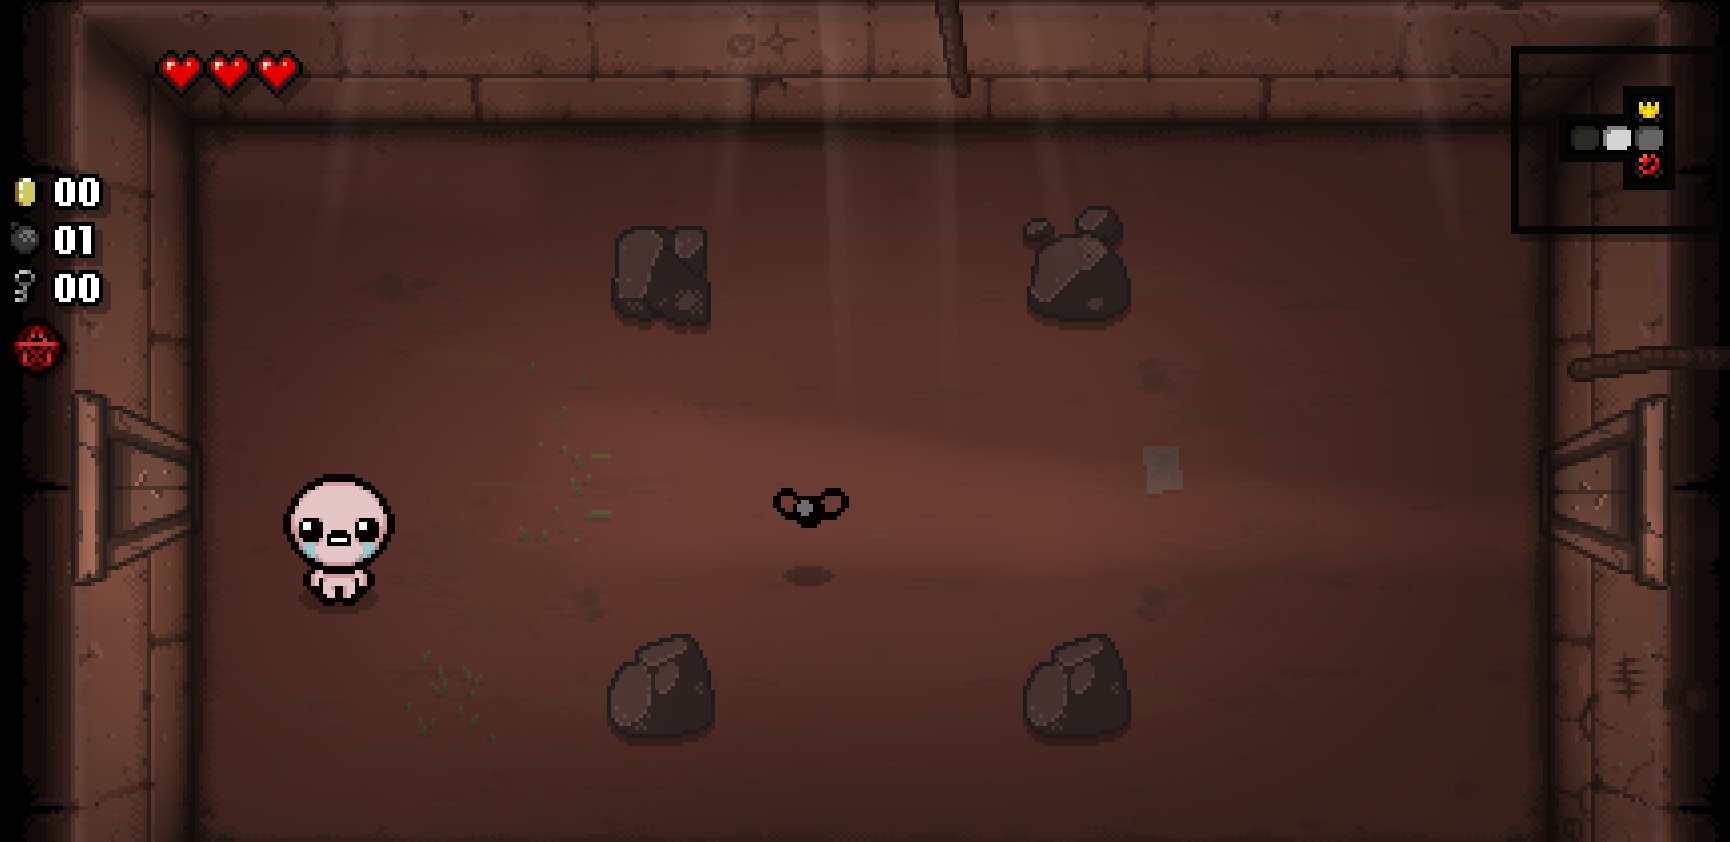
\includegraphics[scale=0.25]{images/research/BOI_Capture.PNG}
                \caption{A screenshot of The Binding of Isaac UI and Map}
                \label{fig:ie_0}
        \end{figure}
        \newpage
        \[\]
        \textbf{Motion Twin's Dead Cells}\\
        Motion Twin created the roguelike dungeon crawler and metroidvania Dead Cells which is released on steam$_{(2)}$. This game is known for its permadeath system and its procedurally generated dungeons.\\
        \\
        The way Dead Cells uses procedural generation interests me as it allows for there to be some fixed attributes to the level whilst still allowing elements of randomness. The developers talk about how they do this in a video devlog$_{(3)}$, here the dev talks about his system of having a fixed structure for each level almost like a skeleton. This skeleton will include stuff like important rooms along the way and how much distance of rooms has to be between them. It then fills in all the spaces for rooms with one of the many handmade rooms made by the developers. After one room has been chosen for a spot this leaves less choice for the other spots as the rooms need to join and flow into each other properly and so as it chooses more of them the structure of the level is determined similar to the wave function collapse algorithm$_{(4)}$.\\
        \\
        This style of generation allows for a unique experience each time whilst keeping a hand crafted and natural feel to the levels that is often lost in other techniques.\\
        \\
        However due to the game being aimed at more hardcore gamers with it being part of the rouguelike genre it can often appear complex and offputting to newer players who dont like the idea of taking multiple runs just to have very little to show for it and not much forward progress in the game. Although the game is a side on game I think that I will use the idea of its procedural generation as inspiration in my product.\\
        \\
        \newpage
        \[\]
        \textbf{Nintendo's Legend Of Zelda Breath of the Wild}\\
        Nintendo created the open-world dungeon crawler which is released on the Nintendo Wii U and the Nintendo Switch$_{(5)}$. This game is known for its open world approach to dungeon crawlers as well as its easy to pick up nature for first time players.\\
        \\
        The game starts with a tutorial that teaches players the mechanics of the game (combat, exploration, and resource gathering). This tutorial helps players into the world without overwhelming them, offering opportunities to learn at their own pace which helps reduce the steep learning curve of other games in the genre. The open-world nature of the game also adds to its replayability, allowing the player to take many different routes to complete the game. However, while the game’s size and allows for alot of replayabilty, the volume of content and time required to explore everything can reduce its effectiveness as a game that can be picked up easily for shorter sessions. Its 3D world and complex systems are features that would be too tricky to implement within the scope of an A-level computer science project. It also does not fully fit the dungeon-crawler genre, particularly as it is less dungeon-focused.\\ 
        \\
        I want to take inspiration from the open-world nature of the game to increase replayability aswell as its approach to tutorials in order to make the learning curve steeper. Ontop of this another feature I would like to take inspiration from is the intuitiveness of the combat system which is easy to learn but hard to master in particular its feature of being able to lock onto enemies.\\
        \\
        Some features I will not be including are the 3D nature and the overall content heaviness aswell as the focus less on dungeon crawling as I believe these would be unnecesary features which would drive up the complexity of the solution both to make and run.\\
        \\
        \newpage
        \[\]   
        \subsection{Limitations and Requirements}
        \begin{tabular}{|c|c|c|}
                \hline
                Requirement&Description&Justification\\
                \hline
                \mr{2}{3cm}{Hardware}&\mr{3}{7cm}{PC or laptop with a Keyboard or Game Controller, minimum of 4GB RAM.\\For Windows/Linux: x86\_32 CPU with SSE2 instructions, any x86\_64 CPU, ARMv8 CPU.\\For Macos: x86\_64 or ARM CPU.\\Integrated graphics with full OpenGL 3.3 support}&\mr{3}{5cm}{These are the requirements for running an executable from Godot. The keyboard(WASD) or controller is needed as the input for the game.}\\
                &&\\
                &&\\
                &&\\
                &&\\
                &&\\
                &&\\
                &&\\
                &&\\
                \hline
                \mr{2}{3cm}{Software}&\mr{2}{7cm}{I will be using the Godot Game Engine and GDScript to program my game.}&\mr{3}{5cm}{I will be using Godot as it is a good 2D game designer that is Free and Open-Source it changes less often than alternatives such as Unity. Ontop of this I have prior experience in Godot and GDScript.}\\
                &&\\
                &&\\
                &&\\
                &&\\
                &&\\
                &&\\
                &&\\
                \hline
                \mr{2}{3cm}{OS Limitations}&\mr{3}{7cm}{For Native Exports:  Windows 7 or newer, macOS 10.13 or newer, Linux distribution released after 2016\\For Web: Firefox 79, Chrome 68, Edge 79, Safari 15.2, Opera 64}&\mr{3}{5cm}{Godot can export easily to any of these platforms and more accessibility is good and I can also export a HTML5 version to be hosted in a website such as https://www.itch.io.}\\
                &&\\
                &&\\
                &&\\
                &&\\
                &&\\
                \hline
                \mr{2}{3cm}{General System Limitations}&\mr{3}{7cm}{A visually or auditory excellent experience}&\mr{3}{5cm}{I do not have the experience with shaders or music and sound effects to add these features to the game in this time and it would make the game requirements higher.}\\
                &&\\
                &&\\
                &&\\
                &&\\
                &&\\
                \hline
        \end{tabular}
        \subsection{Features}
        \subsubsection{Essential Features}
        \begin{tabular}{|c|c|c|c|}
                \hline
                Feature\#&Feature&Description&Justification\\
                \hline
                1&\mr{2}{3cm}{Player Movement and Controls}&\mr{2}{5cm}{The player will control movement using the WASD keys for up, left, down and right respectively. Alternatively they will use the left control stick of a controller.}&\mr{2}{5cm}{This will be used tp navigate around the Dungeon environment and WASD was the most popular control mechanism for the stakeholders with controller close behind. I will also include mouse buttons as a non-mandatory addition.}\\
                &&&\\
                &&&\\
                &&&\\
                &&&\\
                &&&\\
                &&&\\
                &&&\\
                \hline
                2&\mr{2}{3cm}{A Basic Combat System}&\mr{2}{5cm}{The combat system will consist of a primary weapon (melee, magic or ranged) on mouse-1/1 key/X button and a sheild or secondary weapon on mouse-2/2 key/Y button. I will have to implement projectiles and hitboxes for both the player and enemies.}&\mr{2}{5cm}{A basic combat system is essential as it will provide the main difficulty and entertainment within the game.}\\
                &&&\\
                &&&\\
                &&&\\
                &&&\\
                &&&\\
                &&&\\
                &&&\\
                &&&\\
                \hline
                3&\mr{2}{3cm}{Dungeon Environment}&\mr{2}{5cm}{The Dungeon Environment will consist of different shaped rooms with different purposes(e.g. boss room, chest room and shop room.) with hallways connecting inbetween them and a starting room.}&\mr{2}{5cm}{A Dungeon Environment is essential as it is the environment the player will play in.}\\
                &&&\\
                &&&\\
                &&&\\
                &&&\\
                &&&\\
                &&&\\
                \hline
                4&\mr{2}{3cm}{Different Enemies}&\mr{2}{5cm}{The Enemies will consist of a variety of enemies that attack the player with different patterns and have different looks and animations.}&\mr{2}{5cm}{This is essential as it will add variety to the gameplay and each enemy will provide a challenge to the player.}\\\
                &&&\\
                &&&\\
                &&&\\
                &&&\\
                \hline
                5&\mr{2}{3cm}{Appearance and Animations of the Player}&\mr{2}{5cm}{The Player will have a recognisable appearance aswell as animations for all its actions such as walking and fighting}&\mr{2}{5cm}{This is essential as it lets you know where your character is on screen aswell as giving life to the actions the player is performing.}\\\
                &&&\\
                &&&\\
                &&&\\
                \hline
                6&\mr{2}{3cm}{Login System}&\mr{2}{5cm}{Users will be able to login in order to save and reload their progress. The login system will use a username and password with the details being encrypted and stored in an external database. Their will be options for signing in or creating a new account aswell as resetting your password.}&\mr{2}{5cm}{This is an essential feature as saving progress is essential for making the game replayable.}\\
                &&&\\
                &&&\\
                &&&\\
                &&&\\
                &&&\\
                &&&\\
                &&&\\
                &&&\\
                &&&\\
                \hline
                7&\mr{2}{3cm}{User Interface}&\mr{2}{5cm}{A Simple UI that shows status indicators like health, weapons being used, enemy health and magic points.}&\mr{2}{5cm}{This would allow the player to be aware of the characters health and give them the necessary information.}\\
                &&&\\
                &&&\\
                &&&\\
                \hline
        \end{tabular}
        \subsubsection{Desireable Features}
        \begin{tabular}{|c|c|c|c|}
                \hline
                Feature\#&Feature&Description&Justification\\
                \hline
                8&\mr{2}{3cm}{Weapons and a more Advanced Combat System.}&\mr{2}{5cm}{A system of weapons where you can get them from boss drops and potentially shops and a combat system with normal, charged (based on how long you hold down) and special attacks (using a special key).}&\mr{2}{5cm}{Different weapons will allow each player to have a playstyle more customized to them and will allow for the player getting stronger as they progress more. An advanced combat system will allow for a more smooth and enjoyable fighting experience.}\\
                &&&\\
                &&&\\
                &&&\\
                &&&\\
                &&&\\
                &&&\\
                &&&\\
                &&&\\
                \hline
                9&\mr{2}{3cm}{Skill Tree}&\mr{2}{5cm}{A skill tree to unlock unique skills/abilities and get better at using existing skills/weapons. You would gain points from playing the game and can then put them into different areas in order to create a customized character build}&\mr{2}{5cm}{This would further allow the player to choose their own play style and add an element of replayability where you can try going for a different build each time you play. This was also requested by the stakeholders.}\\
                &&&\\
                &&&\\
                &&&\\
                &&&\\
                &&&\\
                &&&\\
                &&&\\
                \hline
                10&\mr{2}{3cm}{Procedurally Generated Dungeons}&\mr{2}{5cm}{The Dungeons would be procedurally generated whilst keeping some amount of structure (e.g. the same amount of distance between posses and key rooms). This would happen through many similar small room sections that can be slotted together in order to make a full dungeon.}&\mr{2}{5cm}{This would create a more engaging game which is different each time you play it and therefore increase replayability exponentially as the different combinations of room increases. This was also requested by the stakeholders.}\\
                &&&\\
                &&&\\
                &&&\\
                &&&\\
                &&&\\
                &&&\\
                &&&\\
                &&&\\
                &&&\\
                \hline
                11&\mr{2}{3cm}{Hidden Areas}&\mr{2}{5cm}{Secret areas that can be unlocked through wasy such as progressing further in the game and coming back or through puzzles/fake walls. Could have secret loot or bosses.}&\mr{2}{5cm}{This feature was highly requested by the stakeholders and would allow for more time spent having fun in the game through finding these areas.}\\
                &&&\\
                &&&\\
                &&&\\
                &&&\\
                &&&\\
                \hline
                12&\mr{2}{3cm}{Inventory Sysetm}&\mr{2}{5cm}{An Inventory to be opened with the E key or the + button through which you will manage equipped weapons, key items, skills and more.}&\mr{2}{5cm}{An Inventory System is an essential feature if we want to add more weapons/weapon types and a skill tree.}\\
                &&&\\
                &&&\\
                &&&\\
                &&&\\
                \hline
                13&\mr{2}{3cm}{Settings and Volume Control}&\mr{2}{5cm}{A settings page to control the volume of noises aswell as the vibrancy of colours.}&\mr{2}{5cm}{One of the Stakeholders has requested this as a feature to help the game be more accessible to them.}\\
                &&&\\
                &&&\\
                &&&\\
                \hline
                14&\mr{2}{3cm}{Difficulty Levels and Hardcore Mode}&\mr{2}{5cm}{A Difficulty level selector which allows the user to up the difficulty(damage the enemies do etc) and a Hardcore Mode which switches the game to a roguelike format with seperate save state to the normal game.}&\mr{2}{5cm}{50\% of the stakeholders are experienced with Dungeon Crawlers so in order to help the game still be reasonably challening for them I will add a difficulty toggle.}\\
                &&&\\
                &&&\\
                &&&\\
                &&&\\
                &&&\\
                &&&\\
                \hline
        \end{tabular}
        \newpage
        \subsection{Success Criteria}
        \begin{tabular}{|c|c|c|c|}
                \hline
                Criteria \# & Abstraction & Success Criteria & Justification\\
                \hline
                1&\mr{2}{2cm}{Players to be able to control and move the player using both the WASD keys and a controller.}&\mr{2}{6cm}{1.1 W key - Forward\\1.2 A key - Left\\1.3 S key - Backward\\1.4 D key - Right\\1.5 Q key - Dash\\1.6 Left Control Stick directional movement corresponds to player movement.}&\mr{2}{4cm}{These Criteria need to be met for the character to be controllable by the player. These specific controls where preffered by the stakeholders.}\\
                &&&\\
                &&&\\
                &&&\\
                &&&\\
                &&&\\
                &&&\\
                &&&\\
                &&&\\
                \hline
                2&\mr{2}{2cm}{Players to be able to have different weapons and attack with them.}&\mr{2}{6cm}{2.1 mouse-1/1 key/X button - Primary Attack\\2.2 mouse-2/2 key/Y button - Secondary Attack\\2.3 Add a basic melee sword\\2.4 Add a basic ranged bow and projectiles\\2.5 Add a basic magic staff and projectiles\\2.6 Add a basic magic staff with area of effect attacks\\2.7 Add a hitbox for the player\\2.8 Add a health bar for the player\\2.9 Add the ability to lock facing an enemy\\2.10 Make sure all attacks go in the correct direction}&\mr{2}{4cm}{These criteria need to be met for a basic combat system to create the main difficulty and entertainment throughout the game}\\
                &&&\\
                &&&\\
                &&&\\
                &&&\\
                &&&\\
                &&&\\
                &&&\\
                &&&\\
                &&&\\
                &&&\\
                &&&\\
                &&&\\
                &&&\\
                &&&\\
                &&&\\
                &&&\\
                \hline
                3&\mr{2}{2cm}{A Dungeon environment for the character to walk around and different rooms}&\mr{2}{6cm}{3.1 Walls that you cannot walk through\\3.2 Floor of the Dungeon\\3.3 Interactive chests for loot\\3.4 Seperate Boss, Chest, Monster and Shop Rooms\\3.5 A room Door that only opens on a certain condition\\3.6 A Dungeon Environment built out of the rooms and corridors}&\mr{2}{4cm}{These Criteria will provide the environment within which the game is played.}\\
                &&&\\
                &&&\\
                &&&\\
                &&&\\
                &&&\\
                &&&\\
                &&&\\
                &&&\\
                &&&\\
                \hline
                4&\mr{2}{2cm}{Different Enemies for the player to face including bosses}&\mr{2}{6cm}{4.1 Enemy Sprites\\4.2 Enemy Pathfinding Abilities\\4.3 Enemy sight range\\4.4 Enemy hitbox\\4.5 Enemy health tracking\\4.6 Melee Enemies\\4.7 Projectile Enemies\\4.8 Boss Enemies with different attack combinations}&\mr{2}{4cm}{These Criterie need to be met in order to provide enemies in order to provide the challenge throughout the game.}\\
                &&&\\
                &&&\\
                &&&\\
                &&&\\
                &&&\\
                &&&\\
                &&&\\
                &&&\\
                \hline
        \end{tabular}
        \newpage
        \begin{tabular}{|c|c|c|c|}
                \hline
                \mr{2}{0.6cm}{}5\mr{2}{0.6cm}{}&\mr{2}{2cm}{Appearance and Animations of the Player}&\mr{2}{6cm}{5.1 Player Sprite\\5.2 Walking Animation\\5.3 Player sprite turns to face the direction of movement\\5.4 Melee Animation\\5.5 Magic Animation\\5.6 Bow Animation}&\mr{2}{4cm}{These Criteria will provide the visual animations so the player knows where they are attacking and moving}\\
                &&&\\
                &&&\\
                &&&\\
                &&&\\
                &&&\\
                &&&\\
                \hline
                6&\mr{2}{2cm}{Login System}&\mr{2}{6cm}{6.1 Password Hashing Algorithm\\6.2 SQL Table to store username and hashed password pairs\\6.3 Ability to create a new account with unique username\\6.4 Validation of Usernames (1$\le$chars$<$15)\\6.5 Validation of passwords (One Special Character, One Number, At least 8 Characters, One upper and lower case character)\\6.6 Input Sanitisation (Removing any escape chars for SQL before sending the command)\\6.7 Ability to log in with an exisiting account and correct password\\6.8 Ability to reset password (If admin account)\\6.9 A general login form which links the other forms}&\mr{2}{4cm}{These Criteria will provide a Login system in order to allow multiple users to login whilst keeping user data secure and accessible by that user.}\\
                &&&\\
                &&&\\
                &&&\\
                &&&\\
                &&&\\
                &&&\\
                &&&\\
                &&&\\
                &&&\\
                &&&\\
                &&&\\
                &&&\\
                &&&\\
                &&&\\
                &&&\\
                &&&\\
                &&&\\
                &&&\\
                &&&\\
                \hline
                7&\mr{2}{2cm}{User Interface}&\mr{2}{6cm}{7.1 Health Bar\\7.2 Magic Points Bar\\7.3 Display of the weapon being used\\7.4 Popup display with enemy health over their head when they get damaged\\7.5 ability to switch between weapons}&\mr{2}{4cm}{These Criteria allow the key information to be displayed to the user aswell as the user being able to change what weapon they have equipped}\\
                &&&\\
                &&&\\
                &&&\\
                &&&\\
                &&&\\
                &&&\\
                \hline
        \end{tabular}
        \newpage
        \begin{tabular}{|c|c|c|c|}
                \hline
                \mr{2}{0.6cm}{}8\mr{2}{0.6cm}{}&\mr{2}{2cm}{Weapons And a More Advanced Combat System}&\mr{2}{6cm}{8.1 Different Styles of melee, magic and ranged weapons\\8.2 Item pick up\\8.3 Boss Drops\\8.4 Shop System that appears throughout levels\\8.5 Charged Attacks (based on how long you hold down)\\8.6 Special attacks}&\mr{2}{4cm}{These Criteria would allow for a more complex combat system to increase differences in the way you play}\\
                &&&\\
                &&&\\
                &&&\\
                &&&\\
                &&&\\
                &&&\\
                &&&\\
                &&&\\
                \hline
                9&\mr{2}{2cm}{Skill Tree}&\mr{2}{6cm}{9.1 UI Menu for the skill tree (Some skills required before others unlocked).\\9.2 Different Branches (Melee, Ranged, Magic, Defense)\\ 9.3 Experience system.\\\tab 9.3.1 Experience gained after \tab killing enemies/bosses\\ \tab 9.3.2 Different experience amounts \tab required for different skills\\9.4 Ability to unlock skills\\9.5 Ability to reset your skill tree}&\mr{2}{4cm}{These Criteria will fulfill a stakeholder desire and will allow the game to have more complexity and replayability}\\
                &&&\\
                &&&\\
                &&&\\
                &&&\\
                &&&\\
                &&&\\
                &&&\\
                &&&\\
                &&&\\
                &&&\\
                \hline
                10&\mr{2}{2cm}{Procedurally Generated Dungeons}&\mr{2}{6cm}{10.1 Creating requirements for each level to satisfy\\10.2 Creating differnt room sections/rooms to peice together\\10.3 Creating the algorithm to generate which room sections are slotted together where.\\10.4 Create an algorithm to peice the sections together to create a fully playable level.\\\tab 10.4.1 Level's generated satisfy \tab length requirements\\\tab 10.4.2 Level's generated contain all \tab the special rooms needed (chest \tab room, secret rooms, etc.)}&\mr{2}{4cm}{These criteria will help to add a ton of replayability to the game aswell as being requested by stakeholders}\\
                &&&\\
                &&&\\
                &&&\\
                &&&\\
                &&&\\
                &&&\\
                &&&\\
                &&&\\
                &&&\\
                &&&\\
                &&&\\
                &&&\\
                &&&\\
                &&&\\
                \hline
                11&\mr{2}{2cm}{Hidden Areas}&\mr{2}{6cm}{11.1 Add mechanics to get into the secret rooms (breakable walls, climbing vines, keys, etc.)\\\tab 11.1.1 Add a hammer to break \tab walls with\\\tab 11.1.2 Add climbing gloves which \tab you need in order to climb vines\\11.2 Add secret Boss and Treasure rooms for behind these obstacles.}&\mr{2}{4cm}{These Criteria will make the game more engaging as well as being requested by the stakeholders}\\
                &&&\\
                &&&\\
                &&&\\
                &&&\\
                &&&\\
                &&&\\
                &&&\\
                &&&\\
                \hline
                12&\mr{2}{2cm}{Inventory System}&\mr{2}{6cm}{12.1 UI for Inventory\\12.2 Storage of Extra weapons and key items (keys, armour, charms, etc)\\12.3 E key to open up the inventory\\12.4 Ability to switch out what Weapons, Armour and charms are equipped.\\}&\mr{2}{4cm}{These criteria will allow for more complexity in the game and more customized and diverse playthrough options which allows for more replayability}\\
                &&&\\
                &&&\\
                &&&\\
                &&&\\
                &&&\\
                &&&\\
                \hline
        \end{tabular}
        \newpage
        \begin{tabular}{|c|c|c|c|}
                \hline
                \mr{2}{0.6cm}{}13\mr{2}{0.6cm}{}&\mr{2}{2cm}{Settings and Volume Control}&\mr{2}{6cm}{13.1 Settings UI with buttons for each setting\\13.2 Ability to control the volume\\13.3 Ability to control the vibrancy of colours in the game.}&\mr{2}{4cm}{These criteria have been requested by stakeholders as a way to increase the accessibility of the game to them}\\
                &&&\\
                &&&\\
                &&&\\
                &&&\\
                \hline
                14&\mr{2}{2cm}{Difficulty Levels and Hardcore Mode}&\mr{2}{6cm}{14.1 A slider for difficulty in the settings menu\\14.2 Increasing difficulty based on the slider\\\tab 14.2.1 Increasing enemy health\\\tab 14.2.2 Decreasing player health\\\tab 14.2.3 Increasing number of \tab enemies\\14.3 A Hardcore mode at maximum difficulty with a seperate save state to the normal game.\\\tab 14.3.1 roguelike features \tab (permadeath, resource \tab management, etc)}&\mr{2}{4cm}{These criteria will allow those of the stakeholders who have more experience in dungeon crawlers aswell as those that have played the game more to up the difficulty and it increases the replayabilty through different challenges.}\\
                &&&\\
                &&&\\
                &&&\\
                &&&\\
                &&&\\
                &&&\\
                &&&\\
                &&&\\
                &&&\\
                &&&\\
                &&&\\
                &&&\\
                &&&\\
                \hline
        \end{tabular}
        \newpage
        \subsection{Computational Methods}
\newpage
\pagestyle{plain}
\section{Design}
        \subsection{Overview}
        \subsubsection{Global Variables}
        I have a couple of main global variable scripts Global, Inventory, Database etc.\\
        \begin{tabular}{|c|c|c|c|}
                \hline
                Source&Identifier&Data Type&Justification\\
                \hline
        \end{tabular}
        \subsubsection{Folder Structure}
        \begin{figure}[H]
                \centering
                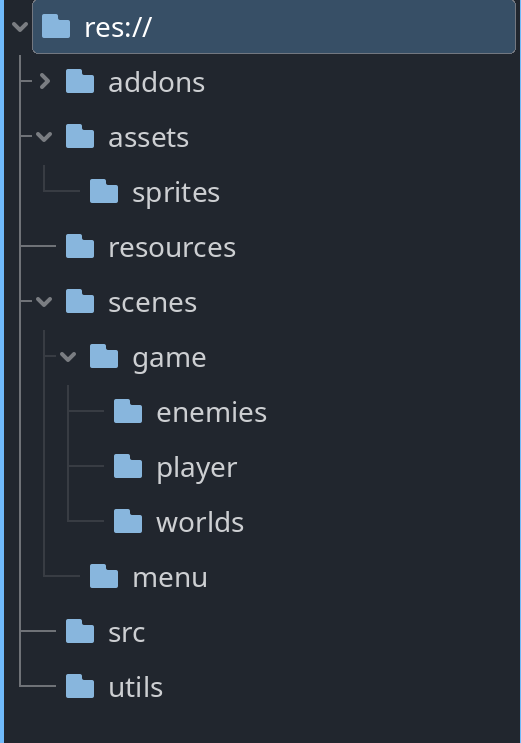
\includegraphics[width = 0.3\textwidth]{images/design/File_System.PNG}
                \caption{Folder Structure}
        \end{figure}
        I chose this folder structure as it will allow me to clearly define where all the different parts of the game are aswell as easily being able to access the closely related parts.\\
        The assets folder will contain all of the external assets, sprites, spritesheets and audio.\\
        The resources folder will contain all of the items (weapons, armour, keys and charms) that I will make to be included in the game.\\
        The scenes folder will contain all the scenes for the menu and the game sorted into their respective folders.\\
        The src folder will contain all of the preloaded scripts for the game.\\
        the utils folder will contain any testing or debugging scripts/scenes to help with the development process.\\
        \subsubsection{Naming Convention}
        For naming I conventions I will adopt the naming conventions already used in godot for ease of integration, readability and consistency with documentation.\\
        The naming conventions are as follows.\\
        \begin{tabular}{|c|c|c|}
                \hline
                Type&Convention&Info\\
                \hline
                File Names&snake\_case&yaml\_parsed.gd\\
                \hline
                Class Names&PascalCase&YAMLParser\\
                \hline
                Node Names&PascalCase&\\
                \hline
                Functions&snake\_case&\\
                \hline
                Variables&snake\_case&\\
                \hline
                Signals&snake\_case& Past tense "door\_opened"\\
                \hline
                Constants&CONSTANT\_CASE&\\
                \hline
        \end{tabular}
        \newpage
        \subsection{Database Design}
        I will be using an SQL Database in order to store the data about my users.\\
        \subsubsection{ERD}
        \begin{figure}[H]
                \centering
                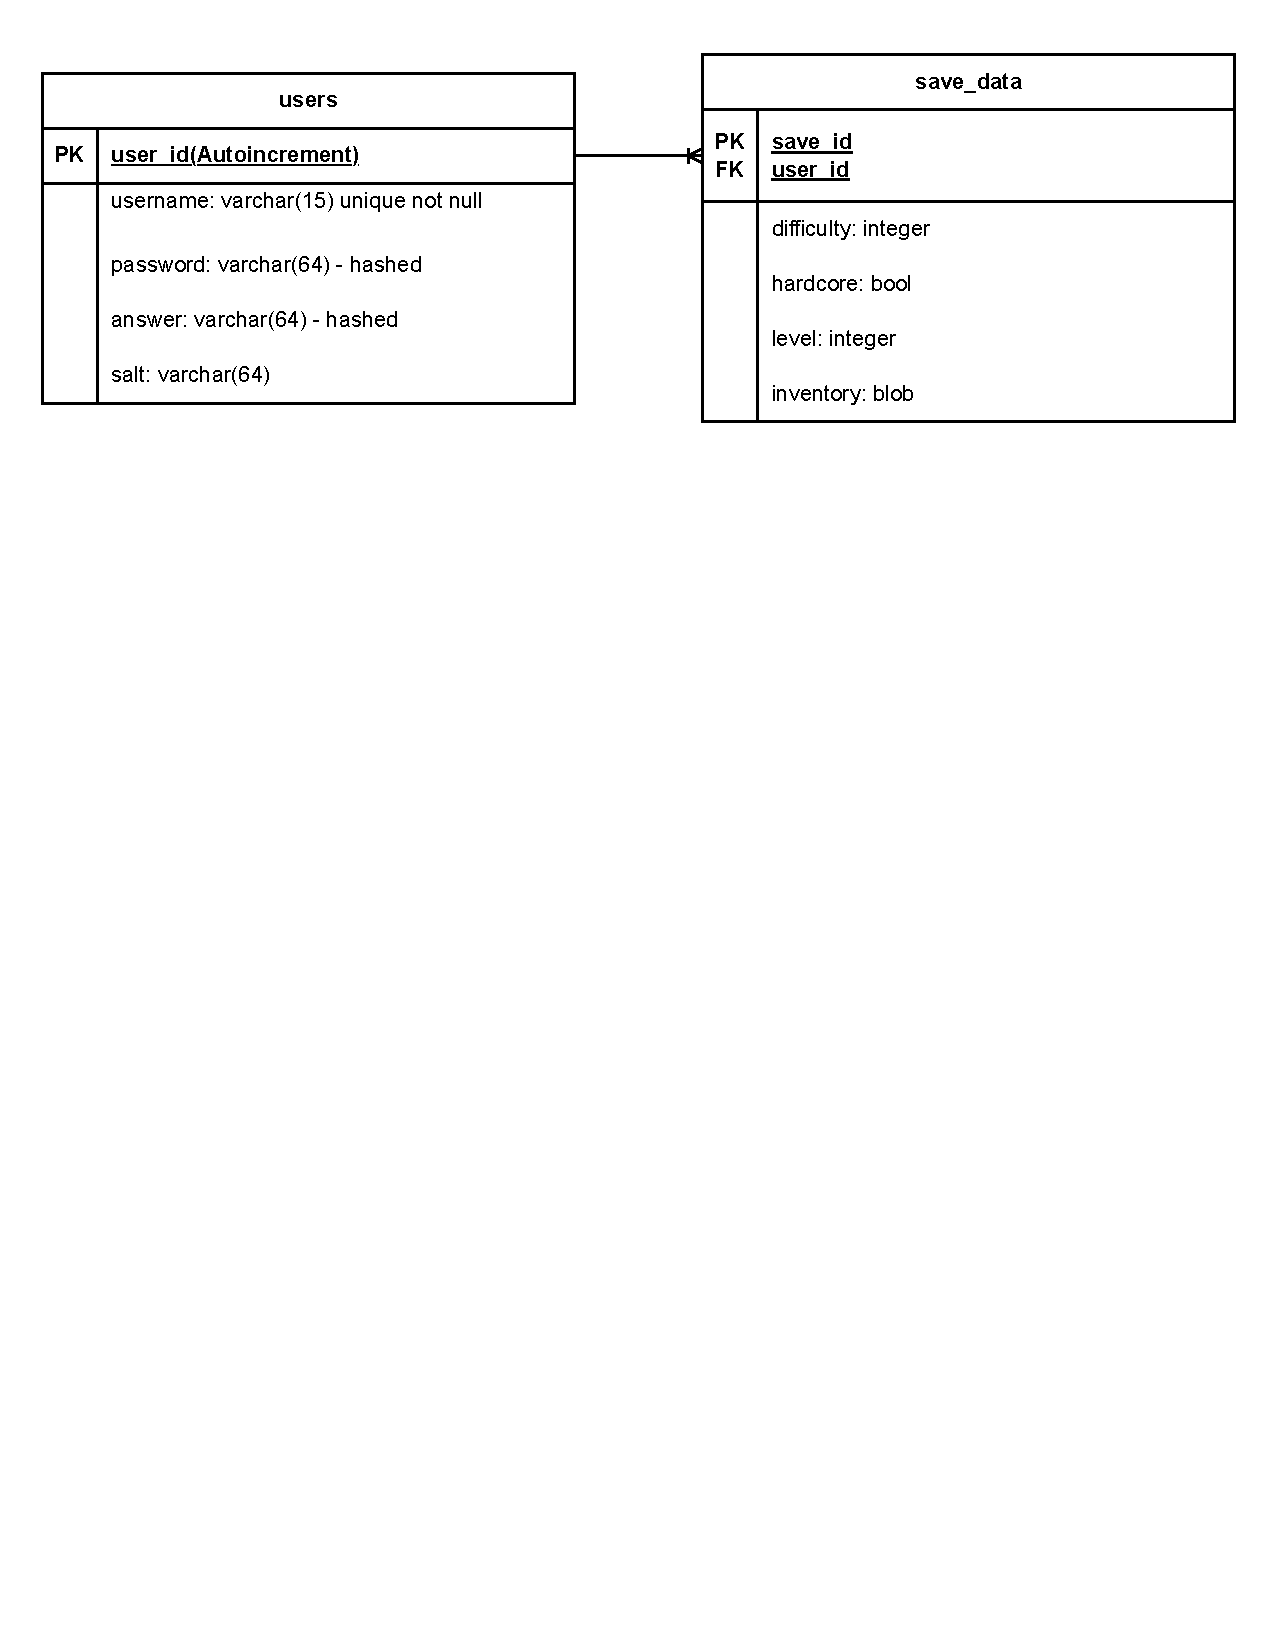
\includegraphics[width=\textwidth, trim = 0 575 0 25, clip]{images/design/Database_Design.pdf}
                \caption{Database Design}
                \label{fig:ie_1}
        \end{figure}
        Figure 2 shows the Database Design:\\
        The users table will be the main table containing all the login details.\\
        Each user will be able to have multiple save instances which will be stored in save data.\\
        Upon designing the inventory I have decided that I will split the inventory into the stored items which I will use a seperate table to store all the equipped 
        \subsubsection{Database Naming Conventions}
        The naming conventions I will adopt for the database is as follows.\\
        \begin{tabular}[pos]{|c|c|c|c|}
                \hline
                Abstract&Convention&Examples&Justification\\
                \hline\
                &&&\\
                Tables&Plural snake\_case&users,save\_data&\mr{7}{4cm}{SQL is case insensitive so with CamelCase it cann't tell the difference between undervalue and underValue}\\
                &&&\\
                \cline{1-3}
                &&&\\
                Fields&Singular snake\_case&inventory\_content, username&\\
                &&&\\
                \cline{1-3}
                &&&\\
                Keys& singular snake\_case\_table\_id&user\_id, save\_data\_id&\\
                &&&\\
                \hline
        \end{tabular}
        
        \subsubsection{SQL Queries}
        I have to write Queries for each of the actions I want to do.\\
        \begin{tabular}{|c|c|c|}
                \hline
                Name&Description/Justification&SQL\\
                \hline
                \mr{2}{3.5cm}{create\_table\_users}&\mr{2}{3cm}{Create's a table for Users if it does not exist.}&\mr{2}{8.5cm}{\texttt{CREATE TABLE IF NOT EXISTS users (\\\tab user\_id INTEGER PRIMARY KEY AUTOINCREMENT,\\\tab username VARCHAR(15) NOT NULL,\\\tab password VARCHAR(64) UNIQUE NOT NULL,\\\tab salt VARCHAR(64) NOT NULL,\\\tab answer VARCHAR(64) NOT NULL\\);}}\\
                &&\\
                &&\\
                &&\\
                &&\\
                &&\\
                &&\\
                &&\\
                \hline
                \mr{2}{3.5cm}{get\_user\_data}&\mr{2}{3cm}{Returns the user data assuming it exists. If it doesnt it will return null.}&\mr{2}{8.5cm}{\texttt{SELECT * FROM users\\WHERE username = ?;}}\\
                &&\\
                &&\\
                &&\\
                \hline
                \mr{2}{3.5cm}{add\_new\_user}&\mr{1}{3cm}{Inserts a new user into users with username, password, challenge question answer and salt}&\mr{2}{8.5cm}{\texttt{--Assume hashed password and answer\\INSERT INTO\\users(username,password,answer,salt)\\VALUES (?,?,?,?);}}\\
                &&\\
                &&\\
                &&\\
                &&\\
                &&\\
                \hline
                \mr{2}{3.5cm}{reset\_password}&\mr{2}{3cm}{Changes a users password}&\mr{2}{8.5cm}{\texttt{--Assume hashed password and answer\\UPDATE TABLE users\\SET invalidCount = 0\\WHERE username = ?}}\\
                &&\\
                &&\\
                &&\\
                \hline
                \mr{3}{3.5cm}{create\_table\_save\_data}&\mr{2}{3cm}{Create's a table for save\_data if it does not exist.}&\mr{2}{8.5cm}{\texttt{CREATE TABLE IF NOT EXISTS save\_data (\\\tab save\_id INTEGER AUTOINCREMENT,\\\tab user\_id INTEGER,\\\tab difficulty INTEGER,\\\tab hardcore INTEGER,\\\tab level INTEGER,\\\tab inventory BLOB DEFAULT x'7b7d'\\);\\--x'7b7d' is the representation of '{}'}}\\
                &&\\
                &&\\
                &&\\
                &&\\
                &&\\
                &&\\
                &&\\
                &&\\
                \hline
                \mr{2}{3.5cm}{add\_new\_save\_data}&\mr{2}{3cm}{Add's new save data for a user.}&\mr{2}{8.5cm}{\texttt{INSERT INTO\\save\_data(user\_id,difficulty,hardcore,level)\\VALUES (?,?,?,?)}}\\
                &&\\
                &&\\
                \hline
                \mr{2}{3.5cm}{get\_save\_data}&\mr{2}{3cm}{Get's the save data with a specific user\_id and save\_id}&\mr{2}{8.5cm}{\texttt{SELECT * FROM users\\WHERE user\_id = ?\\AND save\_id = ?}}\\
                &&\\
                &&\\
                \hline
                \mr{2}{3.5cm}{userSave\_data}&\mr{2}{3cm}{Get's the save data for all entries with a specific user\_id}&\mr{2}{8.5cm}{\texttt{SELECT * FROM users\\WHERE user\_id = ?}}\\
                &&\\
                &&\\
                \hline
                \mr{2}{3.5cm}{update\_save\_data}&\mr{2}{3cm}{updateSave}&\mr{2}{8.5cm}{\texttt{UPDATE save\_data\\SET\\\tab inventory = ?,\\\tab level = ?\\WHERE\\\tab user\_id = ?\\AND save\_id = ?}}\\
                &&\\
                &&\\
                &&\\
                &&\\
                &&\\
                &&\\
                \hline
        \end{tabular}
        \subsection{Login System}
        \subsubsection{Activity Diagram}
        \begin{figure}[H]
                \centering
                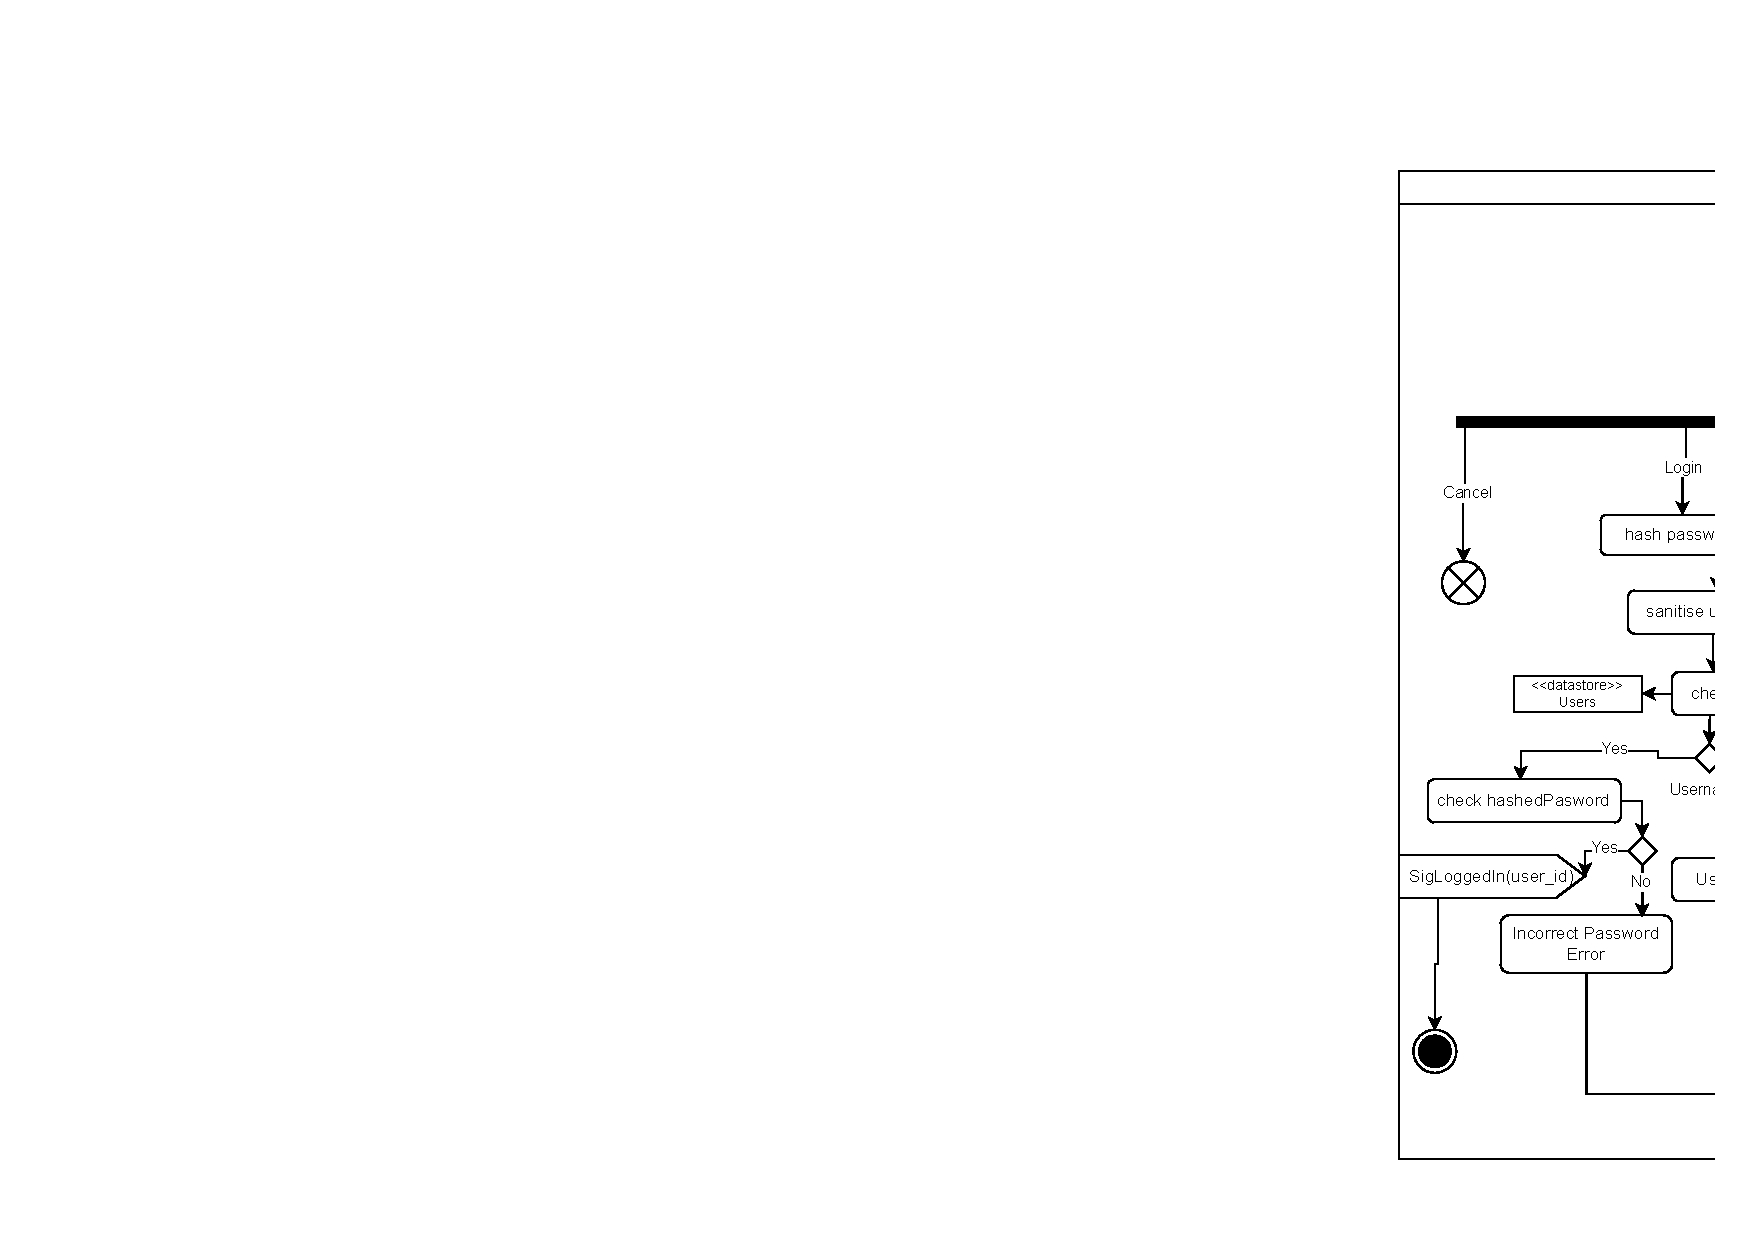
\includegraphics[width=\textwidth, trim = 0 50 0 0, clip]{images/design/Login_System.pdf}
                \caption{Activity Diagram for login forms}
                \label{fig:ie_2}
        \end{figure}
        The login form will allow users to create accounts aswell as login with an existing account and reset a password.\\
        Upon successful login the user will be redirected to the GAME system.\\
        \subsubsection{Algorithms}
        \textbf{hash():}\\
        \begin{python}
def hash(password: str, salt: str):
   hashedPassword = password
   #Repeating a consistent but unpredicatble amount of times
   for x in range(1,6*len(password)+1):
      if x\%2 == 0:
         hashedPassword = sha256(md5(salt[x:]+hashedPassword+salt[:x]))
      else:
         hashedPassword = md5(sha256(hashedPassword[:x]+salt+hashedPassword[x:]))
        return hashedPassword
        \end{python}
        \textbf{removeForm():}\\
        \begin{python}
def changeForm(form1: scene,form2: scene):
   self.remove_child(form1)
   form  = form1.instantiate()
   self.add_child(form)
        \end{python}
        \subsubsection{Mockup Forms}
        \begin{multicols}{3}
                \begin{figure}[H]
                        \centering
                        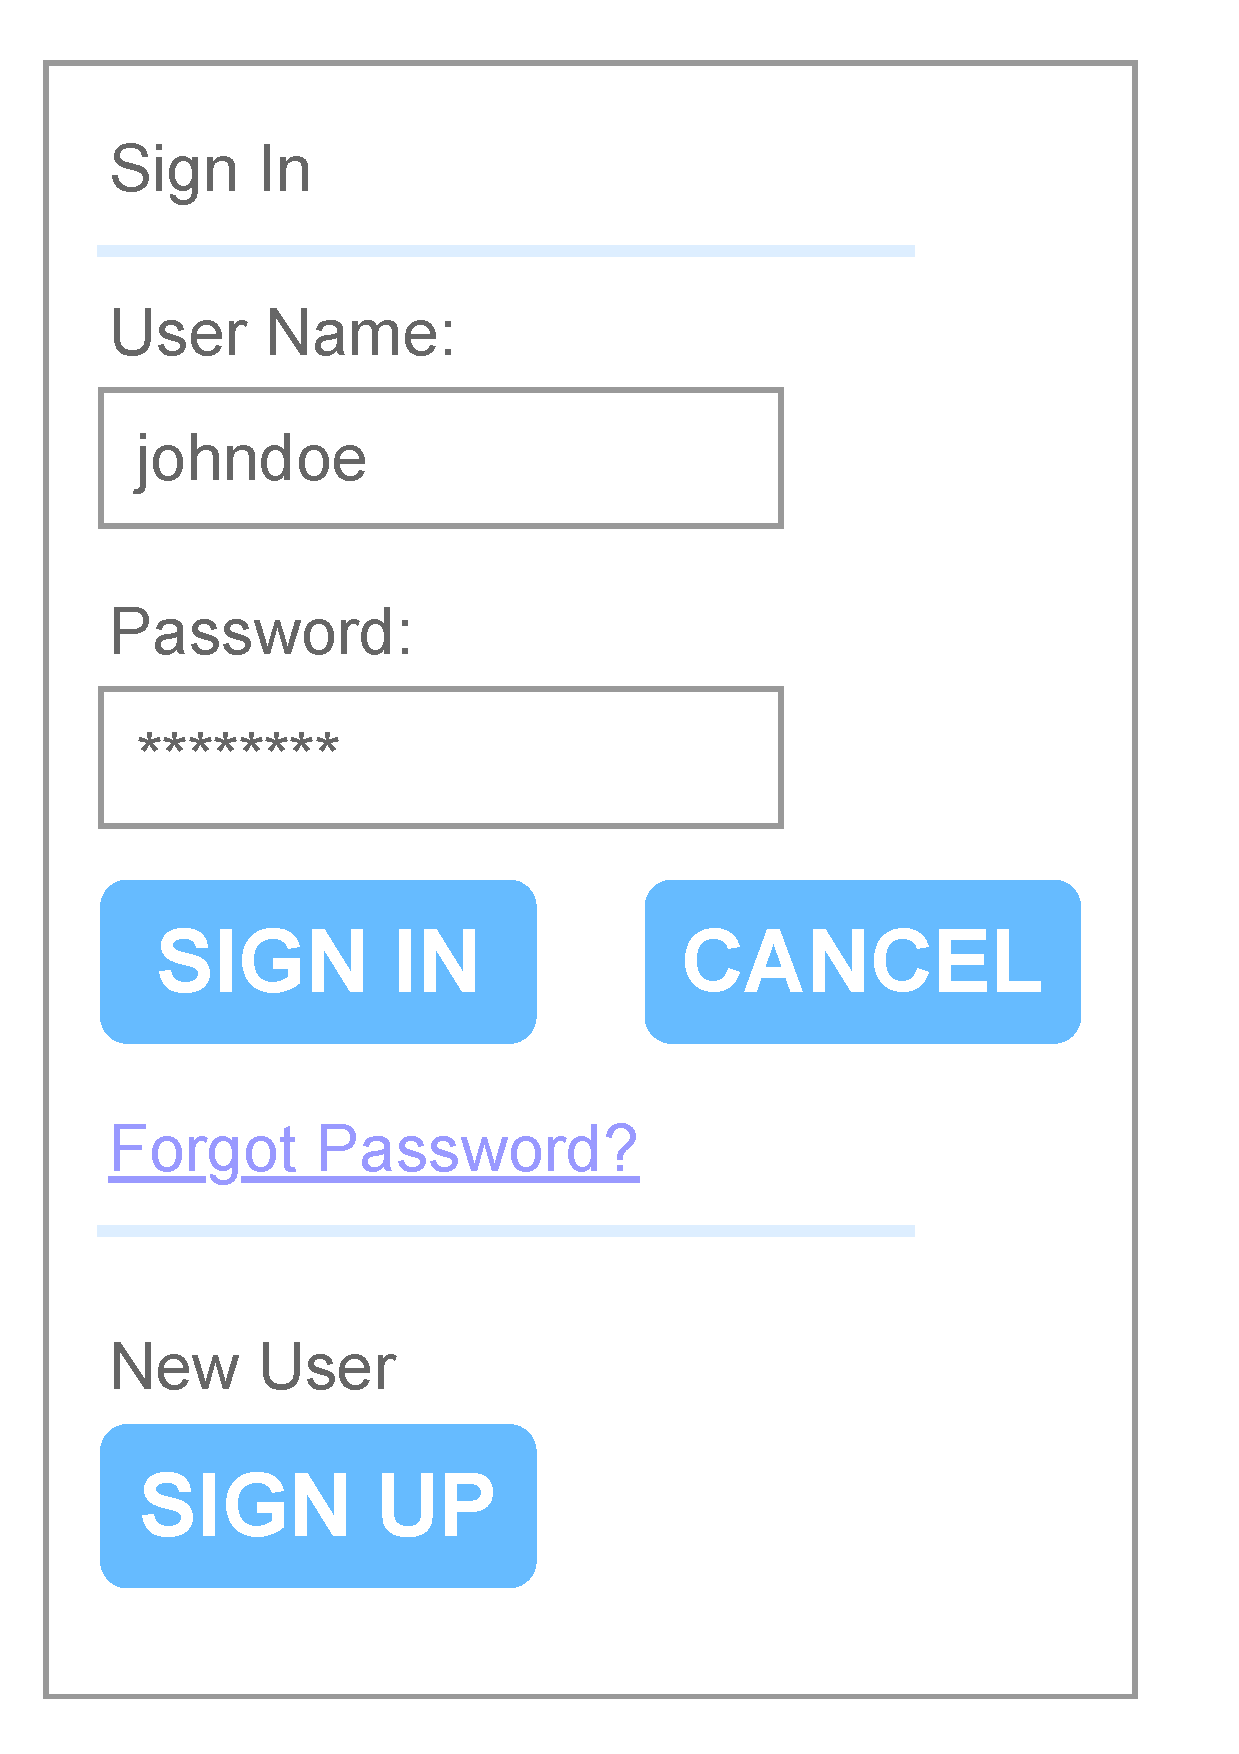
\includegraphics[width = 0.9\columnwidth]{images/design/Login_Form.pdf}
                        \caption{Login Form}
                        \label{fig:ie_3}
                \end{figure}
                \begin{figure}[H]
                        \centering
                        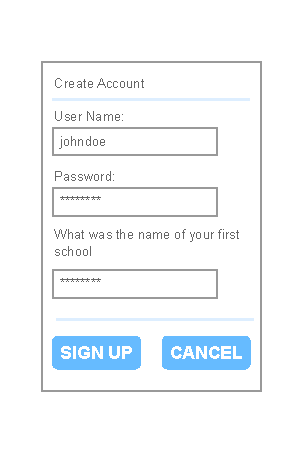
\includegraphics[width = 0.9\columnwidth]{images/design/Sign_Up_Form.pdf}
                        \caption{New Account Form}
                        \label{fig:ie_4}
                \end{figure}
                \begin{figure}[H]
                        \centering
                        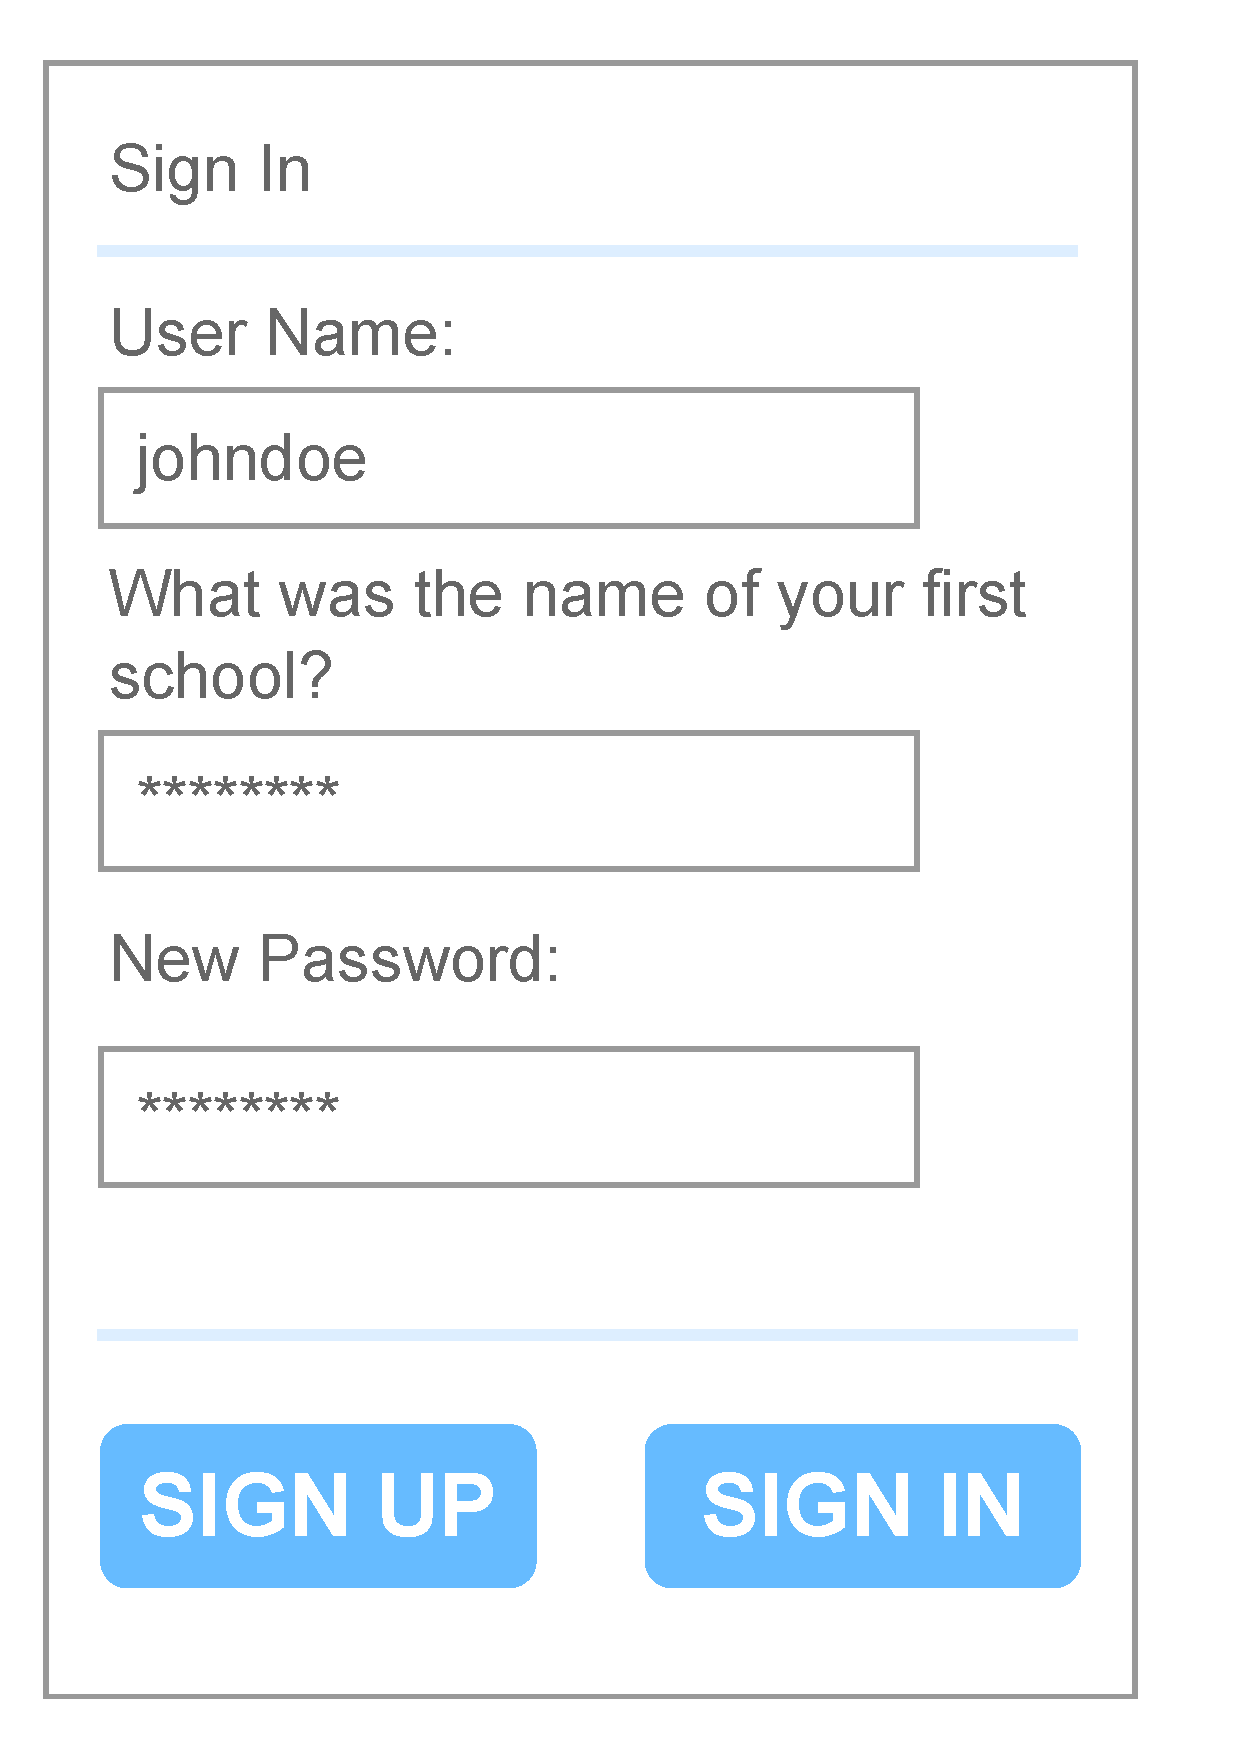
\includegraphics[width = 0.9\columnwidth]{images/design/Reset_Password.pdf}
                        \caption{Reset Password Form}
                        \label{fig:ie_5}
                \end{figure}
        \end{multicols}\[\]
        These forms would be used in order to create an account, reset your password and login.\\
        The Password and Challenge question entries would be starred for privacy.\\
        \newpage
        \subsection{Item Design}
        I will implement the different item types using Godot's resource system. This will allow me to define properties that all items of the same type will share and I can use inheritance to allow classes to derive from a parent class.\\
        The types of items I will aim to implement will be different weapon types, charms/trinkets/amulets, armour and keys.\\
        \subsubsection{Class Diagram}
        \begin{figure}[H]
                \centering
                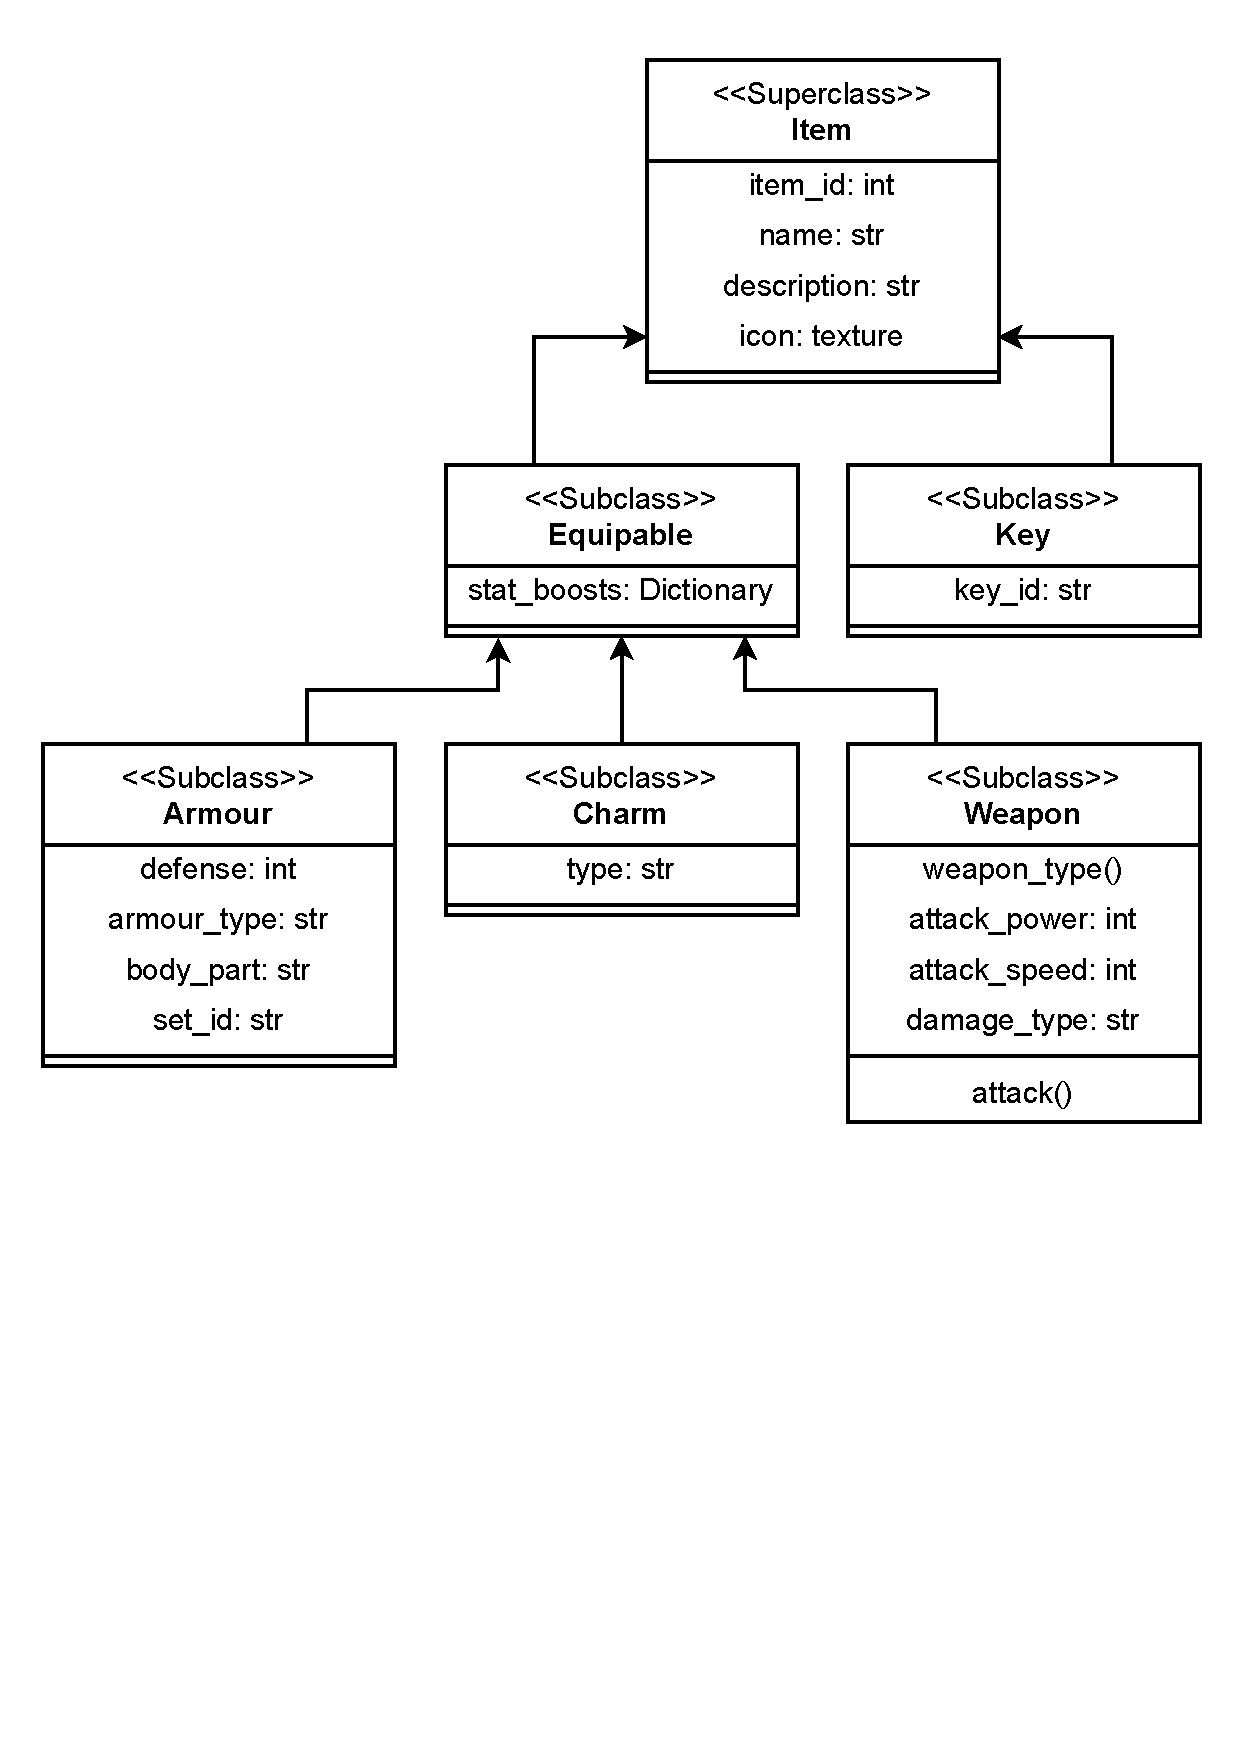
\includegraphics[width = 0.9\columnwidth, clip, trim = 0 270 0 25]{images/design/Item_Class_Diagram.pdf}
                \caption{Player Class Diagram}
                \label{fig:ie_5}
        \end{figure}
        \subsubsection{Algorithms}
        \textbf{attack():}\\
        I will have a number of different weapon types that will have different attacks.\\
        I will implement the attack cooldown through the use of a CooldownTimer(timer node) attached to the player.\\
        Melee:\\
        I will implement the melee attack by creating a variable size hitbox(area2D) scene that can be instantiated as a child of the player in order to detect enemies that would be attacked in the range specified in the resource.\\
        \begin{python}
def attack(owner: node):
   #Load the hitbox scene
   hitbox_scene = load(hitbox_scene_path)
   hitbox_instance = hitbox_scene.instantiate()
   hitbox_instance.range = range
   hitbox_instance.damage = damage

   #Add child
   owner.add_child(hitbox_instance)

   #Hitbox lasts for half a second
   sleep(0.5)
   
   hitbox_instance.queue_free()

        \end{python}
        Ranged:\\
        My Bows and ranged magic weapons will shoot out projectiles.
        \begin{python}
def attack():
   #Load the projectile scene
   projectile_scene = load(projectile_scene_path)
   projectile_instance = projectile_scene.instantiate()
   projectile_instance.damage = damage

   #Add Child
   owner.add_child(projectile_instance)
        \end{python}
        \subsection{Inventory Design}
        My inventory design will cover two main parts the equipped items and the item storage.\\
        \subsubsection{Stored Items}
        I will implement the stored items through a dictionary that stores the item resource and the quantity of it. I will implement add and remove item functions. I will also add a max inventory size.\\
        \subsubsection{Equipped Items}
        I will implement the equipped items through a dictionary where the keys are the slots and the values are what is equipped in that slot. I will also add a equip function to equip an item and an unequip function to unequip the item in a slot.\\
        \subsubsection{Algorithms}
        \textbf{add\_item():}\\
        \begin{python}
def add_item(item: Resource):
   if len(stored_items) > max_inventory_size + 1:
      return null #Indicates that the inventory is full
   else:
      #Checks if you can stack the item and either adds a new entry or stacks it
         if item in stored_items and item.stackable:
            stored_items[item] += 1
         else:
            stored_items[item] = 1
   return item #Indicates success
        \end{python}
        \textbf{remove\_item():}\\
        \begin{python}
def remove_item(item: Resource, quantity: int = 1):
   if item in stored_items:
      if stored_items[item] < quantity:
         return null #Indicates that there is an item quantity error
      stored_items[item] -= quantity #Removes the ammount of that item
      if stored_items[item] == 0:
         stored_items.erase(item)
      return item #Indicates that it was successful
   return null #Indicates that there is an item quantity error
        
        \end{python}
        \textbf{unequip\_item():}\\
        \begin{python}
def unequip_item(slot: str):
   #Checks if there is a slot and item to unequip
   if slot in equipped_items and equipped_items[slot] != null:
      item = equipped_items[slot]
      add_item(item) #Adds the item back to the stored_items
      equipped_items[slot] = null #Sets the slot back to null
      return True
   return False
        \end{python}
        \newpage
        \textbf{equip\_item():}\\
        \begin{python}
def equip_item(item: Resource):
        #Checks if the item is Equipable
        if not(item.is_class(Equipable)):
                return False
        #Gets the slot to equip it inot
        if item.is_class(Armour):
                slot = item.body_part
        elif item.is_class(Weapon):
                slot = "weapon"
        else:
                equipped = false
                #Tries both charm slots
                for slot in ["charm1","charm2"]:
                        if equipped_items[slot] == null and not(equipped):
                                equipped_items[slot] = item #Equips item
                                remove_item(item) #Removes from stored_items
                                equipped = True
                if not(equipped):
                        unequip_item(slot)
                        equipped_items[slot] = item #Equips item
                        remove_item(item) #Removes from stored_items
                return True
        if slot in equipped_items:
                unequip_item(slot)
                equipped_items[slot] = item #Equips item
                remove_item(item) #Removes from stored_items
                return True
        return False      
        \end{python}
        \newpage
        \subsection{Player Character}
        This is my design for the physical player character and sprite.\\
        \subsubsection{Composition}
        \begin{figure}[H]
                \centering
                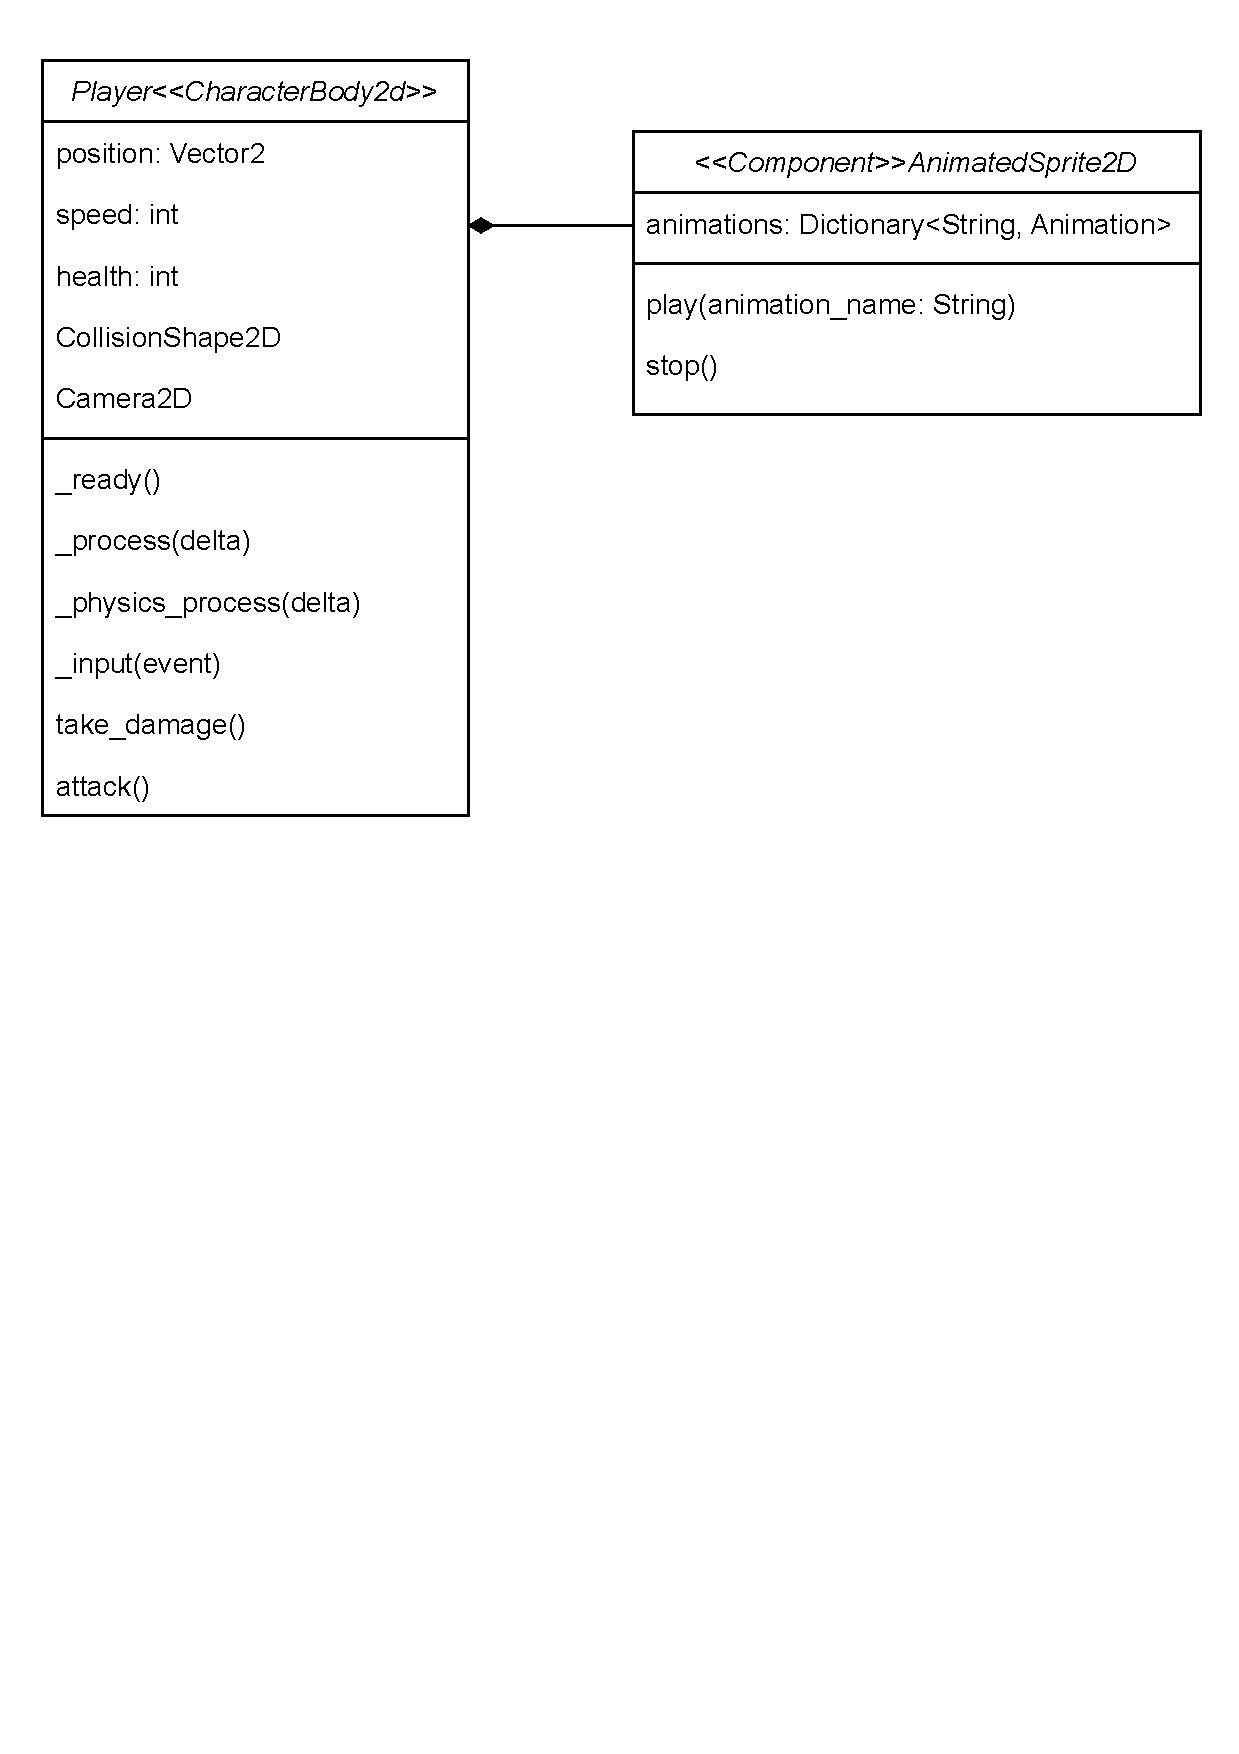
\includegraphics[width = 0.9\columnwidth, clip, trim = 0 450 0 0]{images/design/Player_Class_Diagram.pdf}
                \caption{Player Class Diagram}
                \label{fig:ie_6}
        \end{figure}
        The root node of the player which will contain all the child nodes will be Godot's CharacterBody2D as this will allow for a user controlled physics body. It will then have child nodes of CollisionShape2D(for collision detection), AnimatedSprite2D(for an animated character sprite) and Camera2D(for the player's view window to be centered on).\\
        I have chosen to store the speed and health variables within the player class as they will reset/ be recalculated based of the equipment equipped.\\
        \subsubsection{Algorithms}
        \textbf{\_ready():}\\
        The \_ready() function gets called whenever the player is instantiated in a scene and so it will be used to setup variables and the environment based on existing stuff.\\
        \begin{python}
def _ready():
        #Inventory calculates the speed based on any modifiers equipped.
        speed = Inventory.calc_speed() 
        #Global Script calculates the health based on the player level and any modifiers equipped.
        health = Global.calc_health()
        \end{python}
        \textbf{\_physics\_process(delta):}\\
        The \_physics\_process(delta) function gets called every frame where delta is the time since the last fram and is usually used to deal with movement and physics processes.\\
        \begin{python}
def _physics_process(delta):
   direction = Input.get_vector("left", "right", "up", "down")
   velocity = direction * speed
   move_and_slide()
        \end{python}
        \textbf{\_input(event):}\\
        \begin{python}
def _input(event):
   if event.is_action_pressed('attack'):
      attack()
        \end{python}
\section{Development}
\subsubsection{Database Development}
\section{References}
\begin{tabular}{|c|c|c|c|c|c|}
        \hline
        REF$\#$ &Date&Topic/Abstract&Type&URL or BOOK reference&How I used this\\
        \hline
        1&1/6/24&\mr{2}{3cm}{Research/ Existing Solutions}&\mr{2}{2cm}{video games store, online}& \mr{2}{4cm}{https://store.steampowered\\.com/app/113200/\\The\_Binding\_of\_Isaac}&\mr{2}{3cm}{One of the exisiting solutions I researched.}\\
        &&&&&\\
        &&&&&\\
        \hline
        2&15/6/24&\mr{2}{3cm}{Research/ Existing Solutions}&\mr{2}{2cm}{video games store, online}& \mr{2}{4cm}{https://store.steampowered\\.com/app/588650/\\Dead\_Cells}&\mr{2}{3cm}{One of the existing solutions I researched}\\
        &&&&&\\
        &&&&&\\
        \hline
        3&15/6/24&\mr{2}{3cm}{Research/ Existing Solutions}&\mr{2}{2cm}{youtube video, online}&\mr{2}{4cm}{https://www.youtube.com\\/watch?v\=tyMrRW\-Li\_I}&\mr{2}{3cm}{A dev log for an existing solution.}\\
        &&&&&\\
        &&&&&\\
        \hline
        4&15/6/24&\mr{2}{3cm}{Research/ Existing Solutions}&\mr{2}{2cm}{blog, online}&\mr{2}{4cm}{https://robertheaton.com\\/2018/12/17/wavefunction\-collapse\-algorithm/}&\mr{2}{3cm}{An existing algorithm I researched.}\\
        &&&&&\\
        &&&&&\\
        \hline
        5&25/11/24&\mr{3}{3cm}{Research/ Exisiting Solutions}&\mr{2}{2cm}{video games store, online}&\mr{2}{4cm}{https://store.nintendo.co\\.uk/en/the-legend-of-zelda-breath-of-the-wild-70010000000023}&\mr{2}{3cm}{One of the existing solutions I researched}\\
        &&&&&\\
        &&&&&\\
        &&&&&\\
        \hline
\end{tabular}

\end{document}